Odata ce o cerere de incepere a unei executii a unui workflow este primita de catre crawler, functia Lambda corespunzatoare inceperii executiei (i.e. \textit{"Pornire workflow"}) este invocata. Aceasta creaza si salveaza metadatele necesare in baza de date (e.g. timpul la care a inceput workflow-ul, cu scopul de a putea contoriza cat a durat executia), apoi invoca functia Lambda responsabila pentru initializarea mecanismului de distributie si sincronizare a executiei in paralel a functiilor ce parcurg paginile web. \textit{"Figura 7"} descrie modul in care functia de initializare a unui workflow este utilizata, precum si rolul pe care aceasta il indeplineste in procesul recursiv de crawling.

\begin{figure}[ht]
\begin{center}
	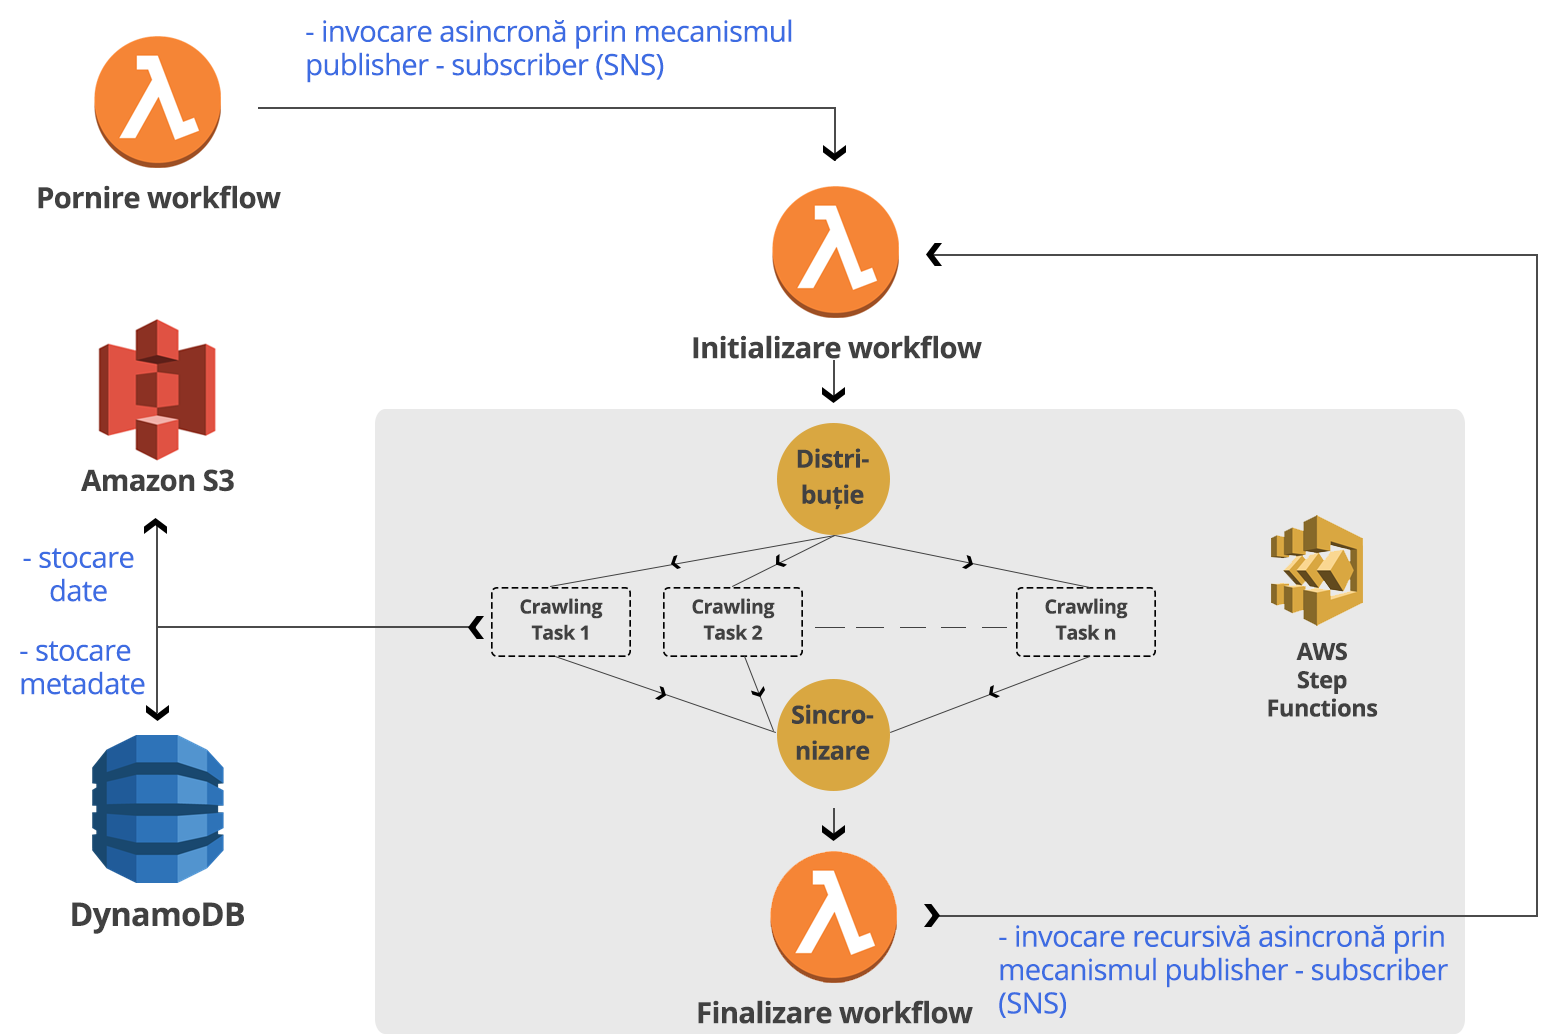
\includegraphics[keepaspectratio, width=1.0\textwidth]{proces-crawling-high-level.png}
	\caption{Arhitectura unui workflow \cite{diagram-icons-sources, aws-icons-source}}\par\medskip 

\end{center}
\end{figure}

Responsabilitatile functiei de initializare a workflow-ului sunt urmatoarele:

\begin{itemize}
	\item{Verificarea nivelului de adancime la care s-a ajuns in urma procesului de crawling si finalizarea workflow-ului, in caz ca nivelul de adancime maxim a fost depasit;}
	\item{Interogatea bazei de date in vederea extragerii task-urilor pentru parcurgerea paginilor web, task-uri ce sunt executate in cadrul automatului orchestrat de catre "AWS Step Functions";}
	\item{Crearea si pornirea automatului finit construit in cadrul "AWS Step Functions", pe baza task-urilor extrase din baza de date. Acest automat este definit prin doua stagii secventiale. Primul stagiu are ca scop orchestrarea distribuita a sarcinilor de crawling executate in paralel, iar cel de-al doilea are ca scop agregarea, interpretarea si salvarea datelor provenite din executia task-urilor concurente.}
\end{itemize}
